MiniTwit follows the server-client architecture, and the server is deployed via a Docker Swarm, which consists of virtual machines (aka 'droplets') on DigitalOcean. Data, such as user data, messages, and followers, is stored in a PostgreSQL database, which is also hosted on DigitalOcean. \\
In the swarm, we have manager-nodes and worker-nodes. The only services allowed to run on the managers are Prometheus and Dozzle (more about the swarm services in section \ref{scaling}). Figure \ref{fig:DeployDiagram} shows a specification-level deployment diagram showing how MiniTwit is deployed on a worker node.
\begin{figure}[h]
\centering
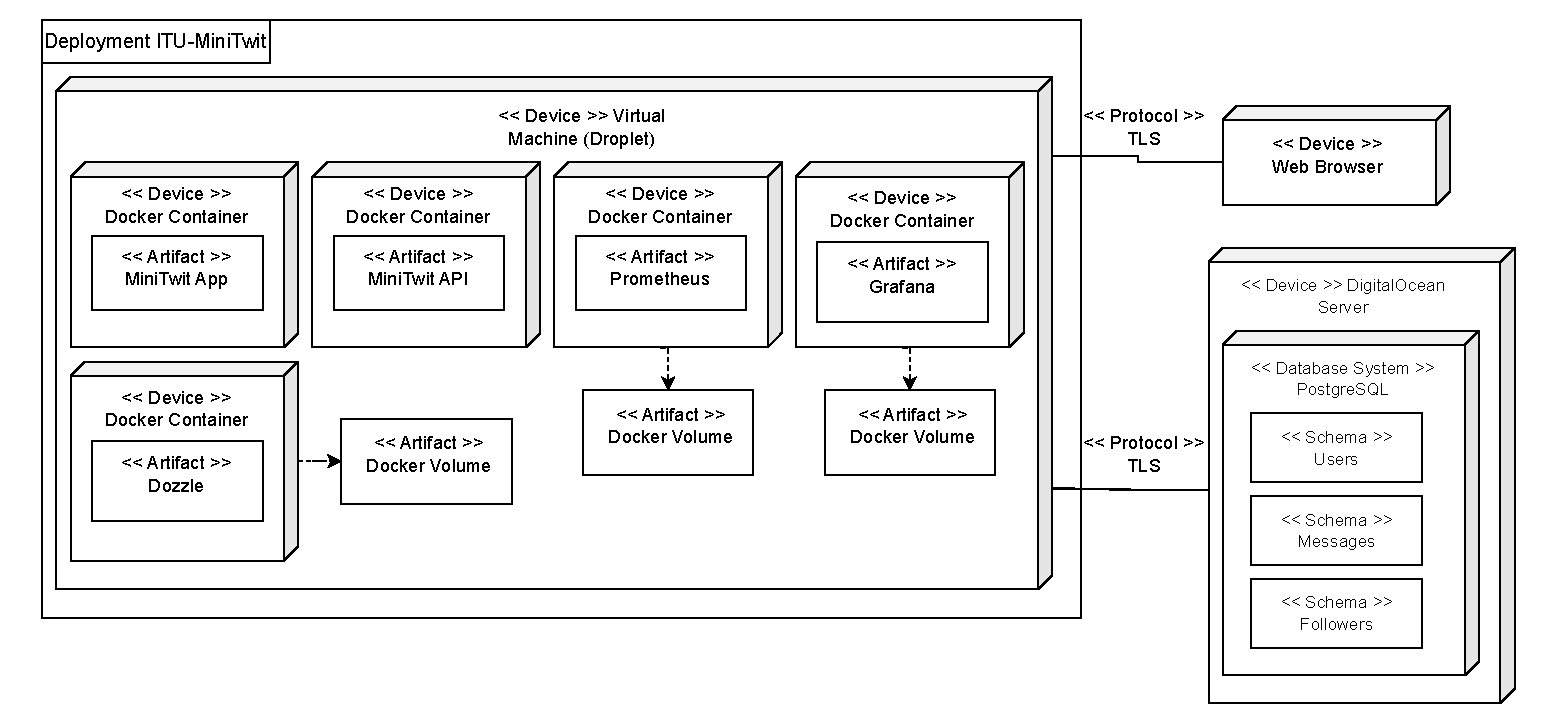
\includegraphics[scale=0.5, center]{images/DeployUMLDraft(1).pdf}
\caption{Deployment Diagram of MiniTwit on a worker node}
\label{fig:DeployDiagram}
\end{figure}